\documentclass{article}
% set up the page formatting
\usepackage[a4paper, portrait, margin=2.5cm]{geometry}
\usepackage{multicol}
\usepackage{fancyhdr}
\usepackage{graphicx}
\usepackage{float}
% editable bits
\title{CS261 Group 29 Requirement Analysis}
\author{Add your names here}
\date{January 2025}
\fancyfoot[L]{Requirement Analysis}
\fancyfoot[R]{\thepage}

\begin{document}
\maketitle

\section{Introduction}
% Justifies the need for the system and outlines what it will do.
Dorset Software has beeen contracted to create a system used for the modelling 
of traffic junctions based on various parameters. The system will provide 
data about how each of these functions impacts the performance of a given 
junction and allow for comparison of various sets of parameters to help 
determine the best option for a given junction. As a group we have been given 
the task of the development of this system along with the documentation and 
project management.

\section{System Architecture}
% Presents a high-level overview of the system, showing distribution of functions across system modules.
% Make sure that the requirements are in order of priority
\begin{figure}[H]
    \centering
    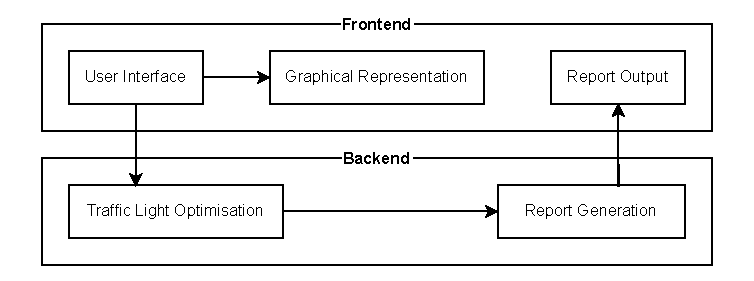
\includegraphics[width=0.5\linewidth]{System architecture.drawio.pdf}
    \caption{System Architecture Diagram}
    \label{system architecture}
\end{figure}

\section{System Requirements Specification}
% Describes functional and non-functional requirements.
\subsection{Requirement 1}
\subsubsection{Customer Facing}
The user must be able to input the rate of traffic flow from 
each direction to each other direction via text fields (one per traffic flow) 
in the User Interface (UI).
\subsubsection{Developer Facing}
\begin{itemize}
  \item The system must accept input from the text fields, parse the input to 
  determine if each traffic flow is a valid number, and, if all traffic flows 
  are valid, allow the simulation to be ran.
  \item Priority: must
  \item Verification: running the simulation with one set of valid traffic 
  flow rates in the text fields, running it again with a different set in 
  the same fields and verifying the junction efficiency metrics have changed, 
  and then trying to run the simulation with an invalid value in at least one 
  text field (e.g. “TEST” for Eastbound Traffic Flow Exiting West)
  \item Traceability: Input Parameters section in the specification
\end{itemize}

\subsection{Requirement 2}
\subsubsection{Customer Facing}
The user must be able to adjust the following settings for each 
road entering the junction, affecting the results of the simulation: how many 
lanes there are (1 to 5), whether there is a left-turn lane, bus lane, cycle 
lane (all mutually exclusive, the latter two requiring separate traffic flow rates) 
or none of those three, whether there is a pedestrian crossing (requires the duration 
of time the crossing is active and the number of crossing requests per hour), 
and the traffic light sequencing priority (0 to 4, 0 meaning no priority, 4 
meaning highest priority).
\subsubsection{Developer Facing}
\begin{itemize}
  \item For each junction configuration, the system must take into account 
  its specific settings, adjusting the calculations performed by the simulation 
  for that specific configuration
  \item Priority: must
  \item Verification: run a simulation with default parameters (2 lanes per 
  road entering the junction, equal priority on all lights, and all other 
  settings set to off/No) as a reference, and then run a simulation per setting 
  with that setting adjusted, showing the results of each simulation is different 
  from the reference.
  \item Traceability: Configurable Parameters section in the specification
\end{itemize}

\subsection{Requirement 3}
\subsubsection{Customer Facing}
After running the simulation, for each junction configuration, 
the user must be provided with the following three junction efficiency metrics 
per road entering the junction, as well as an overall score generated from the 
three metrics for the whole configuration: average wait time, maximum wait time, 
and maximum queue length.
\subsubsection{Developer Facing}
\begin{itemize}
  \item When the simulation is ran, for each junction configuration, the system 
  must take the configuration and the input traffic flow rates (shared across all 
  configurations) and calculate the average wait time, maximum wait time and 
  maximum queue length per direction entering the junction, as well as combine 
  these metrics to calculate an overall score for the whole configuration
  \item Priority: must
  \item Verification: run the simulation once with two different configurations 
  or twice with a single configuration and different traffic flows, and verify 
  that there is a difference between the metrics and overall score of the 
  configurations/simulation runs
  \item Traceability: Output section in the specification
\end{itemize}

\subsection{Requirement 4}
\begin{itemize}
  \item The system must allow for comparison of one or more sets of input parameters against the metrics defined in section \ref{requirements_user}
\end{itemize}

\subsection{Requirement 5}
\subsubsection{Customer Facing}
The user must be able to select whether cars drive on the left-hand side of 
the road or right-hand side, affecting the graphical representation of the junction
configuration and the results of the simulation (junction efficiency metrics).
\subsubsection{Developer Facing}
\begin{itemize}
  \item The system must take into account the setting determining which side of
  the road cars drive on, affecting the calculations of the simulation and how 
  the junction configuration is displayed on the UI.
  \item Priority: should
  \item Verification: switching cars from driving on the left-hand side to the 
  right-hand side and observing a change in the graphical representation, running 
  the simulation, then switching cars back to driving on the left-hand side and 
  running the simulation again, observing a change in the graphical representation 
  and a difference in the junction efficiency metrics
  \item Traceability: Constraints and Assumptions section in the specification, included 
  as a unique selling point of our software
\end{itemize}

\subsection{Requirement 6}
\subsubsection{Developer Facing}
\begin{itemize}
  \item The system must take into account the distance between the entrance and exit 
  points of each junction configuration. So, for example, a left turn from the 
  leftmost lane of a road has a shorter distance than a right turn from the leftmost 
  lane of the road (assuming driving on the left-hand side of the road)
  \item Priority: should
  \item Verification: run the simulation on a specific example where at least one of 
  the metrics should be affected when the distance is taken into account (e.g. one 
  road has 100vph exiting right, preventing another road’s 100vph from exiting to its
  own right and another road’s 100vph from exiting ahead such that these two do not 
  interfere with each other)
  \item Traceability: Constraints and Assumptions section in the specification, included 
  as a unique selling point of our software
\end{itemize}

\subsection{Requirement 7}
\begin{itemize}
  \item The system will show graphical representation of the junction based on the parameters entered (left turn lanes, bus lanes etc). This makes it easier for the user to understand how exactly their settings affect the design of a junction and if they are what they intended.
  \item Priority: Should-have 
  \item Verification: The representation can be generated as an image and then that image compared to a generated image that has been checked to be correct. This would be able to be unit tested but should also be used  with functional testing.
\end{itemize}

\subsection{Requirement 8}
\subsubsection{Customer Facing}
When the simulation is ran, if a certain setting is configured, then the best 
possible set of junction settings based on the same input traffic flows and the 
junction efficiency metrics will be displayed alongside the other junction 
configurations the user created.
\subsubsection{Developer Facing}
\begin{itemize}
  \item When the simulation is ran, if the setting is configured, then the best 
  possible junction configuration (and its results) for the set of input traffic 
  flows must be determined and output along with the results of the junction 
  configurations created by the user
  \item Priority: could
  \item Verification: run the simulation without the setting configured and verify 
  no extra junction configuration is displayed, then run the simulation again with 
  the setting configured, and verify that the extra junction configuration is displayed 
  and that it is the most effective configuration based on its efficiency metrics
  \item Traceability: while not directly specified, this requirement could be traced back 
  to the Output section, where it states that the client’s main objective when using 
  the software is “to identify the most effective configuration of the traffic junction”
\end{itemize}

\subsection{Requirement 9}
\subsubsection{Customer Facing}
When the simulation is ran, the user should be able to select a certain exit and display the amount of traffic going into other exits via a sankey diagram junction.
\subsubsection{Developer Facing}
\begin{itemize}
  \item When the simulation is ran, the user should be able to click on an exit and see the amount of traffic flowing into the other exits from the selected exit where the volume flowing in into the other exit is proportional to the parameter size
  \item Priority: could
  \item Verification: Select an exit and check whether the amount of traffic flowing is proportional to the input sizes. Repeat for the other exits
  \item Traceability: while not directly specified, the requirement could be traced back to the Output section where the customer wants to be able to “identify the most effective configuration of the traffic junction”. By adding this, the user could see how the traffic flows into other exits via a graphical interface that will change depending on the user's inputs.
\end{itemize}

\subsection{Requirement 10}
\subsection{Developer Facing}
\begin{itemize}
  \item The sytem must allow users to compare the metric of different junction configurations side by side in a table or graph format.
  \item Must
  \item Verification: Simulate two different junction configurations with the same inputs and verify that the results are displayed in a side by side comparison
\end{itemize}

\subsection{Requirement 11}
\subsection{Developer Facing}
\begin{itemize}
  \item The system must validate user input in real time, identifying invalid entries and providing clear feedback to guide the user toward correction.
  \item Must
  \item Verification:
  \begin{itemize}
      \item Enter a valid number in a traffic flow field and ensure the simulation proceeds without error.
      \item Enter an invalid value (e.g., “abc” or a negative number) and verify that the system highlights the field, displays an error message, and prevents the 
      simulation from starting until the error is corrected.
      \item Leave a required field empty and ensure the system displays a warning, specifying the field that needs attention.
  \end{itemize}
\end{itemize}

\subsection{Requirement 12}
\subsection{Developer Facing}
\begin{itemize}
  \item The system must provide user-friendly error messages for invalid inputs or system failures. These messages should clearly explain the issue in
  non-technical terms for the user, while also logging technical details for debugging purposes.
  \item Must
  \item Verification: 
  \begin{itemize}
      \item Trigger a known error, such as submitting invalid traffic flow rates, and verify that the system displays a user-friendly error message with
      details like the affected field and suggested resolution.
      \item Simulate a system failure and confirm that a technical error message is logged for debugging, while the user sees a generic failure message.
  \end{itemize}
\end{itemize}



\subsection{Non-functional Requirements}

\section{Project Philosophy}
\subsection{Team Roles}
% playing to strengths blah blah
Our team is comprised of the following members:

\begin{itemize}
  \item Krister - Backend 
  \item Josh - Frontend and Backend 
  \item Antoni - Backend 
  \item Eshan -  Frontend
  \item Thomas - Frontend
  \item Ani - Video, Frontend and Backend
\end{itemize}

As a team we have been meeting once a week on Wednesdays and will continue to do 
so until the end of the project. When recording the Dragon's Den video presentation 
we will allocate some more time as well as making sure that someone who's familiar 
with video editing software is able to fully focus on the video to make it as good
as possible. 

Together we have decided to forgo a project manager and opt for regular meetings 
with a shared understanding of the goals, if anyone has any concerns about the group 
structure or work distribution then this can be brought up at the whole group meeting 
to everyone, everyone is an equal on the team.

\subsection{Development Philosophy}
% waterfall/reuse driven development
We will utilise a hybrid approach combining the main themes of Waterfall with a 
reuse oriented methodology for the software development part of the project. We 
have strict deadlines for each part of the waterfall cycle. The following are 
those timelines, they are spaced to allow sufficient time for each section as 
well as allowing for the whole team to review each stage and make any corrections 
we deem necessary. 

%should be in the design  as part of software development methodology
\begin{itemize}
  \item Requirement Analysis
        - 22nd January
  \item Planning and Design
        - 29th January
  \item Implementation and testing
        - 19th February
  \item Dragon's Den Video and Final Report
        - 26th February
\end{itemize}

Between these stages we will be writing the deliverables as a team alongside,
during the weekly meetings we will check the progress of the various documents,
giving feedback about the changes and any things that should be altered to best 
fit the requirements and plan of the project.

\end{document}
